\documentclass[UTF8]{ctexart}

\usepackage{geometry}
\usepackage{titling}
\usepackage{titlesec}
\usepackage{paralist}
\usepackage{footnote}
\usepackage{marginnote}
\usepackage{enumerate}
\usepackage{autobreak}
\usepackage{amsmath, amssymb, amsthm}
\usepackage{mathtools}
\usepackage{bbm}
\usepackage{cite}
\usepackage{graphicx}
\usepackage{subcaption}
\usepackage{physics}
\usepackage{siunitx}
\usepackage{tikz}
\usepackage[compat=1.1.0]{tikz-feynhand}
\usepackage[ruled, vlined, linesnumbered, noend]{algorithm2e}
\usepackage[colorlinks]{hyperref} % linkcolor=black, anchorcolor=black, citecolor=black, filecolor=black
\usepackage[most]{tcolorbox}
\usepackage{caption}
\usepackage{prettyref}

\geometry{left=3.18cm,right=3.18cm,top=2.54cm,bottom=2.54cm}
\titlespacing{\paragraph}{0pt}{1pt}{10pt}[20pt]
\setlength{\droptitle}{-5em}

\DeclareMathOperator{\timeorder}{\mathcal{T}}
\DeclareMathOperator{\diag}{diag}
\DeclareMathOperator{\legpoly}{P}
\DeclareMathOperator{\primevalue}{P}
\DeclareMathOperator{\sgn}{sgn}
\newcommand*{\ii}{\mathrm{i}}
\newcommand*{\ee}{\mathrm{e}}
\newcommand*{\const}{\mathrm{const}}
\newcommand*{\suchthat}{\quad \text{s.t.} \quad}
\newcommand*{\argmin}{\arg\min}
\newcommand*{\argmax}{\arg\max}
\newcommand*{\normalorder}[1]{: #1 :}
\newcommand*{\pair}[1]{\langle #1 \rangle}
\newcommand*{\fd}[1]{\mathcal{D} #1}

\newrefformat{sec}{第\ref{#1}节}
\newrefformat{note}{注\ref{#1}}
\newrefformat{fig}{图\ref{#1}}
\newrefformat{alg}{算法\ref{#1}}
\newrefformat{back}{背景知识\ref{#1}}
\newrefformat{info}{资料框\ref{#1}}
\newrefformat{warn}{注意事项\ref{#1}}

\usetikzlibrary{arrows,shapes,positioning}
\usetikzlibrary{arrows.meta}
\usetikzlibrary{decorations.markings}
\tikzstyle arrowstyle=[scale=1]
\tikzstyle directed=[postaction={decorate,decoration={markings,
    mark=at position .5 with {\arrow[arrowstyle]{stealth}}}}]
\tikzstyle ray=[directed, thick]
\tikzstyle dot=[anchor=base,fill,circle,inner sep=1pt]

% Algorithm setting
\renewcommand{\algorithmcfname}{算法}
% Python-style code
\SetKwIF{If}{ElseIf}{Else}{if}{:}{elif:}{else:}{}
\SetKwFor{For}{for}{:}{}
\SetKwFor{While}{while}{:}{}
\SetKwInput{KwData}{输入}
\SetKwInput{KwResult}{输出}
\SetArgSty{textnormal}

\tcbuselibrary{skins, breakable, theorems}

%\renewcommand{\emph}[1]{\textbf{#1}}
\newcommand*{\concept}[1]{{\textbf{#1}}}


\newcommand{\Ztwo}{$\mathbb{Z}_2$}

% Cite: superscript, [1]
%\makeatletter
%\renewcommand\@citess[1]{\textsuperscript{[#1]}}
%\makeatother

\title{自旋和费米子体系的蒙特卡洛模拟}
\author{吴晋渊 18307110155}

\begin{document}

\maketitle

\section{蒙特卡洛模拟概述}

\subsection{马尔可夫链蒙特卡洛}

凝聚态物理中,经常需要计算哈密顿量为$H$的平衡态统计系统在温度$T$下的各种物理量的期望值
\begin{equation}
    \expval{O} = \frac{1}{Z} \sum_{\text{configuration $\mathcal{C}$}} \ee^{- \beta H[\mathcal{C}]} O[\mathcal{C}], \quad Z = \sum_{\mathcal{C}} \ee^{- \beta H[\mathcal{C}]},
    \label{eq:sampling}
\end{equation}
其中逆温$\beta = 1 / T$。%
\footnote{
    由于在研究有效模型,我们可以使用自然单位制以节约篇幅。
}%
这个期望值计算一般来说是难以完成的,因为设体系有$N$个格点,每个格点的状态有$n$种取值范围,则一共有$n^N$种可能的系统构型。
对量子系统,情况更加棘手,此时$\mathcal{C}$应当理解为体系的一个能量本征态,而$H$的能量本征态——或者也可以说是零温性质——一般而言是无法求出的。

蒙特卡洛模拟是一种数值解决以上问题的方法。计算物理中通常所说的蒙特卡洛方法一般都是马尔可夫链蒙特卡洛方法,即构造马尔可夫链
\begin{equation}
    \cdots \rightarrow \mathcal{C}_{n-1} \rightarrow \mathcal{C}_n \rightarrow \mathcal{C}_{n+1} \rightarrow \cdots,
\end{equation}
保证这个马尔可夫链各态历经(即从一个状态出发,必有概率非零的一条链能够到达任何一个其它状态),且满足如下细致平衡条件:
\begin{equation}
    p(\mathcal{C} \to \mathcal{D}) p(\mathcal{C}) = p(\mathcal{D} \to \mathcal{C}) p(\mathcal{D}), \quad p(\mathcal{C}) \coloneqq \frac{1}{Z} \ee^{- \beta H[\mathcal{C}]}
\end{equation}
或者更加宽松的全局平衡条件(细致平衡的马尔可夫链一定也是全局平衡的,但反之不然)
\begin{equation}
    p(\mathcal{C}) = \sum_\mathcal{D} p(\mathcal{D}) p(\mathcal{D} \to \mathcal{C}).
\end{equation}
此时,随机过程的理论保证了该马尔可夫链收敛时,状态$\mathcal{C}$出现的概率一定是$p(\mathcal{C})$。
这样,将一个已经收敛的马尔可夫链运行一段时间,并各个时间点处$O$的值,计算算术平均,就得到了$\expval{O}$的近似值,运行时间越长,近似效果也越好。

\subsection{Binning技术}

从$\mathcal{C}_{n-1}$到$\mathcal{C}_n$的过程称为\concept{更新}。由于常规的算法的更新都是相对局域的,$\mathcal{C}_{n-1}, \mathcal{C}_n, \mathcal{C}_{n+1}$这些靠得较近的状态会较为相似。将$\{\mathcal{C}_n\}$序列——从而$\{O_n\}$序列——看成一个信号,我们说这个信号存在\concept{自关联(autocorrelation)}。
在计算$\expval{O}$近似值时,如果更新步数在马尔可夫链的自关联长度以内,$\expval{O}$的近似值将出现严重的系统性偏差,对其方差的估算也是非常不准确的,可能严重偏低(例如$O$是系统能量,相似的构型能量相似)或偏高(如$\mathcal{O}$是\emph{反铁磁}序参量,翻转自旋即改变符号)。

最为安全的做法是,在$\{\mathcal{C}_n\}$序列中每隔自关联长度采样一次,而丢弃其它所有的$\mathcal{C}_n$。
这样能够保证物理量的平均值和方差足够精确,但浪费较大。一种折中的做法是,将$\{\mathcal{C}_n\}$划分成一系列等长的区间(称为\concept{bin}),每个bin的长度长于自关联长度,计算这个bin内的$O$的平均值,将其作为这个bin内的$O$的代表,然后计算各个bin中的$O$的平均值的平均值和方差。
这个过程称为\concept{binning}。实际上,可以不实际测自关联长度而拿一段较长的$\{\mathcal{C}_n\}$序列直接做binning,如果发现调整bin长度得到的方差基本不变,那么说明无论是单个bin的长度还是整个$\{\mathcal{C}_n\}$序列的长度都已经足够了。
文献\cite{landau2021guide}对binning技术有详细的讨论。

\subsection{Metropolis更新}

所谓\concept{Metropolis更新}是指一次翻转一个格点上的自由度的更新方法。常见的Metropolis更新可以分成两种,一种是先随机选取一个格点$\vb*{i}$,尝试将其上的自由度$s_{\vb*{i}}$从一个值$s_{\vb*{i}}$切换到$s_{\vb*{i}}'$,真的做这一更新的概率(称为\concept{接受率})是
\begin{equation}
    \begin{aligned}
        p(\mathcal{C} \to \mathcal{C}' | \text{$\vb*{i}$ is chosen}) &= \begin{cases}
            1, &\quad H[\mathcal{C}] \geq H[\mathcal{C}'], \\
            {p(\mathcal{C}')} / {p(\mathcal{C})}, &\quad H[\mathcal{C}] < H[\mathcal{C}'],
        \end{cases} \\
        &= \min (1, p(\mathcal{C}') / p(\mathcal{C})) \\
        &= p(u \leq p(\mathcal{C}') / p(\mathcal{C}) ),
    \end{aligned}
    \label{eq:metropolis-update}
\end{equation}
其中$u$是均匀分布在0和1之间的一个随机变量。在这种更新策略下,设构型$\mathcal{C}$和$\mathcal{C}'$仅仅在格点$\vb*{i}$上有差别,那么有
\begin{equation}
    \begin{aligned}
        \frac{p(\mathcal{C} \to \mathcal{C}')}{p(\mathcal{C}' \to \mathcal{C})} &= \frac{p(\text{$\vb*{i}$ is chosen}) p(\mathcal{C} \to \mathcal{C}' | \text{$\vb*{i}$ is chosen})}{p(\text{$\vb*{i}$ is chosen}) p(\mathcal{C}' \to \mathcal{C} | \text{$\vb*{i}$ is chosen})} \\
        &= \begin{cases}
            \frac{1}{p(\mathcal{C}) / p(\mathcal{C}')} , &\quad H[\mathcal{C}] \geq H[\mathcal{C}'], \\
            \frac{p(\mathcal{C}') / p(\mathcal{C})}{1}, &\quad H[\mathcal{C}] < H[\mathcal{C}'], 
        \end{cases} \\
        &= \frac{p(\mathcal{C}')}{p(\mathcal{C})},
    \end{aligned}
\end{equation}
于是细致平衡条件成立。各态历经条件的成立是显然的。因此,这个更新策略是正确的。

另一种更加常见的Metropolis更新是依照顺序选择格点$\vb*{i}$,然后根据\eqref{eq:metropolis-update}做更新。此时,一步更新应该理解成遍历一趟全部格点,对单个格点的更新由于依赖于格点位置,不能看成马尔可夫链的一个步骤。
此时我们有
\begin{equation}
    p(\mathcal{C} \to \mathcal{C}') = p(\mathcal{C} \to \mathcal{C}|_{s_{1} \to s_{1}'}) p(\mathcal{C}|_{s_{1} \to s_{1}'} \to \mathcal{C}|_{s_{1, 2} \to s_{1, 2}'}) \cdots p(\mathcal{C}|_{s_{1, 2, \ldots, N-1} \to s_{1, 2, \ldots, N-1}'} \to \mathcal{C}'),
\end{equation}
以及
\begin{equation}
    p(\mathcal{C}' \to \mathcal{C}) = p(\mathcal{C}' \to \mathcal{C}|_{s_{2, 3, \ldots, N} \to s'_{2, 3, \ldots, N}}) p(\mathcal{C}|_{s_{2, 3, \ldots, N} \to s'_{2, 3, \ldots, N}} \to \mathcal{C}|_{s_{3, \ldots, N} \to s'_{3, \ldots, N}}) \cdots p(\mathcal{C}|_{s_N \to s_{N}'} \to \mathcal{C}),
\end{equation}
显然,两者之比并无分子分母的共同因子可以约分。事实上,这种更新方式是可能会违反细致平衡条件的(例如,一维伊辛模型在固定次序做Metropolis更新时就违反细致平衡条件\cite{manousiouthakis1999strict}),虽然它仍然保证全局平衡条件。
这种更新方法甚至可能出现不各态历经的情况,不过不各态历经的情况仅限于翻转某个自由度时概率不发生变化时,如果这种情况真的出现了,那么可以以\SI{50}{\percent}对\SI{50}{\percent}的概率决定是否翻转,这样的话,各态历经条件仍然是成立的。
有关的讨论见\cite{brugge2021convergence}。%
\footnote{
    此文献关于平衡条件的说法有误,它似乎认为加入\SI{50}{\percent}对\SI{50}{\percent}的概率后,得到的马尔可夫链满足细致平衡条件,但正如前面所说,这是不对的,我们只能够保证全局平衡条件。
}%

Metropolis更新以外尚有其它更新方式,如在系统接近二级相变点时,由于系统关联长度很大,Metropolis更新非常缓慢,此时应当使用集团更新方法。
有关的讨论可见\cite{binder1993monte}。

\subsection{量子蒙特卡洛}

对量子系统,虽然原则上可以先将$H$做严格对角化,然后将系统的能量本征态视作系统构型并做蒙特卡洛取样,但这两个步骤都极其困难。
大的多体系统的严格对角化基本上是不现实的,能量本征态具有复杂的内部结构,亦没有简明的方法能够做局部的修改而从一个能量本征态切换到另一个能量本征态。
一种做量子蒙特卡洛的方法是\concept{离散路径积分蒙特卡洛}。
记系统中的全体自由度为$s$,我们对算符$\ee^{- \beta H}$做Trotter分解,即近似认为
\[
    Z = \trace \ee^{- \Delta \tau H} \ee^{- \Delta \tau H} \cdots \ee^{- \Delta \tau H},
\] 
并在两个$\ee^{- \Delta \tau H}$之间插入正交完备关系,则有
\begin{equation}
    Z = \sum_{s_0, s_1, \cdots, s_{N_\tau - 1}} \mel{s_0}{\ee^{- \Delta \tau H}}{s_1} \mel{s_1}{\ee^{- \Delta \tau H}}{s_2} \cdots \mel{s_{N_\tau - 1}}{\ee^{- \Delta \tau H}}{s_0}, \quad N_\tau \coloneqq \beta / \Delta \tau.
    \label{eq:discrete-path-integral}
\end{equation}
这个配分函数的形式和一个$d+1$维格子上的\emph{经典}统计系统的配分函数的形式一致,其中,温度变化带来的影响体现在这个$d+1$维经典统计系统多出来的维度的有限尺度效应上。
显然,\eqref{eq:discrete-path-integral}是一个离散路径积分,统计物理中通常将这个多出来的维度称为\concept{虚时间},从而\eqref{eq:discrete-path-integral}称为平衡态下的虚时间路径积分,和零温下的实时间路径积分相对应。
直观地看,多出的这个维度体现了体系不仅具有热涨落(蒙特卡洛更新时场构型的变化),也具有量子涨落(不同虚时间点场构型有不同的值),量子涨落驱动体系“自己”的时间演化,而热涨落表示系统和外界(热库)相互作用导致的涨落。

离散路径积分蒙特卡洛有更为优化的版本:世界线蒙特卡洛。如果能够从离散路径积分的场构型中识别出某种“粒子”,即可将场构型的虚时间演化化归为粒子的世界线,通过局部调整世界线的形状、增减粒子即可做蒙特卡洛模拟。
除了离散路径积分蒙特卡洛以外,还有随机级数展开、连续时间路径积分蒙特卡洛等方法。
关于这些方法的介绍可参考\cite{assaad2008world};本实验主要讨论费米子系统的行列式蒙特卡洛(determinant quantum Monte Carlo, DQMC)方法。

\section{经典伊辛模型的Metropolis蒙特卡洛模拟}

\subsection{Metropolis更新}

经典伊辛模型
\begin{equation}
    Z = \sum_{\{\sigma_{\vb*{i}}\}} \ee^{- \beta H[\{\sigma_{\vb*{i}}\}]}, \quad H[\{\sigma_{\vb*{i}}\}] = - J \sum_{\pair{\vb*{i}, \vb*{j}}} \sigma_{\vb*{i}} \sigma_{\vb*{j}} - h \sum_{\vb*{i}} \sigma_{\vb*{i}}, \quad \sigma_{\vb*{i}} = \pm 1
\end{equation}
是重要的统计模型,它在凝聚态物理中的意义主要是演示铁磁性的起源,但它已经在广阔得多的领域内得到了应用。
此处我们使用Metropolis更新来对经典伊辛模型做蒙特卡洛模拟。
由于最终出现在配分函数中的参数仅有$\beta J$和$\beta h$,在以下推导中,我们可以将$\beta$吸收进$J$和$h$中,从而实际模拟时保持$J, h$不变,调节$T$等效为按照因子$\beta$成比例缩放$J$和$h$,将保持$J, T$不变,调节$h$等效为保持$J$不变,按照$\beta \Delta h$的大小变动$h$。

\begin{figure}
    \centering
    

\tikzset{every picture/.style={line width=0.75pt}} %set default line width to 0.75pt        

\begin{tikzpicture}[x=0.75pt,y=0.75pt,yscale=-1,xscale=1]
%uncomment if require: \path (0,300); %set diagram left start at 0, and has height of 300

%Straight Lines [id:da7900688343051199] 
\draw [color={rgb, 255:red, 74; green, 144; blue, 226 }  ,draw opacity=0.5 ][line width=1.5]    (102,134) -- (168,134) ;
%Straight Lines [id:da22968837564615008] 
\draw [color={rgb, 255:red, 74; green, 144; blue, 226 }  ,draw opacity=0.5 ][line width=1.5]    (168,68) -- (168,134) ;
%Straight Lines [id:da13157986418239975] 
\draw [color={rgb, 255:red, 74; green, 144; blue, 226 }  ,draw opacity=0.5 ][line width=1.5]    (168,134) -- (168,200) ;
%Straight Lines [id:da801148560717611] 
\draw [color={rgb, 255:red, 74; green, 144; blue, 226 }  ,draw opacity=0.5 ][line width=1.5]    (168,134) -- (234,134) ;
%Straight Lines [id:da6808408566351207] 
\draw [color={rgb, 255:red, 0; green, 0; blue, 0 }  ,draw opacity=0.5 ]   (234,68) -- (234,134) ;
%Straight Lines [id:da35890973732003917] 
\draw [color={rgb, 255:red, 0; green, 0; blue, 0 }  ,draw opacity=0.5 ]   (168,68) -- (234,68) ;
%Straight Lines [id:da7296987791011087] 
\draw [color={rgb, 255:red, 0; green, 0; blue, 0 }  ,draw opacity=0.5 ]   (168,200) -- (234,200) ;
%Straight Lines [id:da07996474880653448] 
\draw [color={rgb, 255:red, 0; green, 0; blue, 0 }  ,draw opacity=0.5 ]   (102,134) -- (102,200) ;
%Straight Lines [id:da27575937842607634] 
\draw [color={rgb, 255:red, 0; green, 0; blue, 0 }  ,draw opacity=0.5 ]   (234,134) -- (234,200) ;
%Straight Lines [id:da38042419134786254] 
\draw [color={rgb, 255:red, 0; green, 0; blue, 0 }  ,draw opacity=0.5 ]   (102,68) -- (102,134) ;
%Straight Lines [id:da504469642986344] 
\draw [color={rgb, 255:red, 0; green, 0; blue, 0 }  ,draw opacity=0.5 ]   (102,68) -- (168,68) ;
%Straight Lines [id:da16311920253073486] 
\draw [color={rgb, 255:red, 0; green, 0; blue, 0 }  ,draw opacity=0.5 ]   (102,200) -- (168,200) ;
%Shape: Circle [id:dp12660612618234834] 
\draw  [draw opacity=0][fill={rgb, 255:red, 255; green, 255; blue, 255 }  ,fill opacity=1 ] (154.5,134) .. controls (154.5,126.54) and (160.54,120.5) .. (168,120.5) .. controls (175.46,120.5) and (181.5,126.54) .. (181.5,134) .. controls (181.5,141.46) and (175.46,147.5) .. (168,147.5) .. controls (160.54,147.5) and (154.5,141.46) .. (154.5,134) -- cycle ;
%Shape: Circle [id:dp8272795300855829] 
\draw  [color={rgb, 255:red, 80; green, 227; blue, 194 }  ,draw opacity=0.3 ][fill={rgb, 255:red, 255; green, 255; blue, 255 }  ,fill opacity=1 ][line width=1.5]  (220.5,134) .. controls (220.5,126.54) and (226.54,120.5) .. (234,120.5) .. controls (241.46,120.5) and (247.5,126.54) .. (247.5,134) .. controls (247.5,141.46) and (241.46,147.5) .. (234,147.5) .. controls (226.54,147.5) and (220.5,141.46) .. (220.5,134) -- cycle ;
%Shape: Circle [id:dp37957345707032264] 
\draw  [color={rgb, 255:red, 80; green, 227; blue, 194 }  ,draw opacity=0.3 ][fill={rgb, 255:red, 255; green, 255; blue, 255 }  ,fill opacity=1 ][line width=1.5]  (154.5,68) .. controls (154.5,60.54) and (160.54,54.5) .. (168,54.5) .. controls (175.46,54.5) and (181.5,60.54) .. (181.5,68) .. controls (181.5,75.46) and (175.46,81.5) .. (168,81.5) .. controls (160.54,81.5) and (154.5,75.46) .. (154.5,68) -- cycle ;
%Shape: Circle [id:dp8415187405246769] 
\draw  [draw opacity=0][fill={rgb, 255:red, 255; green, 255; blue, 255 }  ,fill opacity=1 ] (220.5,68) .. controls (220.5,60.54) and (226.54,54.5) .. (234,54.5) .. controls (241.46,54.5) and (247.5,60.54) .. (247.5,68) .. controls (247.5,75.46) and (241.46,81.5) .. (234,81.5) .. controls (226.54,81.5) and (220.5,75.46) .. (220.5,68) -- cycle ;
%Shape: Circle [id:dp70137316267554] 
\draw  [draw opacity=0][fill={rgb, 255:red, 255; green, 255; blue, 255 }  ,fill opacity=1 ] (88.5,68) .. controls (88.5,60.54) and (94.54,54.5) .. (102,54.5) .. controls (109.46,54.5) and (115.5,60.54) .. (115.5,68) .. controls (115.5,75.46) and (109.46,81.5) .. (102,81.5) .. controls (94.54,81.5) and (88.5,75.46) .. (88.5,68) -- cycle ;
%Shape: Circle [id:dp36470096186038825] 
\draw  [draw opacity=0][fill={rgb, 255:red, 255; green, 255; blue, 255 }  ,fill opacity=1 ] (88.5,200) .. controls (88.5,192.54) and (94.54,186.5) .. (102,186.5) .. controls (109.46,186.5) and (115.5,192.54) .. (115.5,200) .. controls (115.5,207.46) and (109.46,213.5) .. (102,213.5) .. controls (94.54,213.5) and (88.5,207.46) .. (88.5,200) -- cycle ;
%Shape: Circle [id:dp7844046903427413] 
\draw  [color={rgb, 255:red, 80; green, 227; blue, 194 }  ,draw opacity=0.3 ][fill={rgb, 255:red, 255; green, 255; blue, 255 }  ,fill opacity=1 ][line width=1.5]  (154.5,200) .. controls (154.5,192.54) and (160.54,186.5) .. (168,186.5) .. controls (175.46,186.5) and (181.5,192.54) .. (181.5,200) .. controls (181.5,207.46) and (175.46,213.5) .. (168,213.5) .. controls (160.54,213.5) and (154.5,207.46) .. (154.5,200) -- cycle ;
%Shape: Circle [id:dp4884199260348432] 
\draw  [draw opacity=0][fill={rgb, 255:red, 255; green, 255; blue, 255 }  ,fill opacity=1 ] (220.5,200) .. controls (220.5,192.54) and (226.54,186.5) .. (234,186.5) .. controls (241.46,186.5) and (247.5,192.54) .. (247.5,200) .. controls (247.5,207.46) and (241.46,213.5) .. (234,213.5) .. controls (226.54,213.5) and (220.5,207.46) .. (220.5,200) -- cycle ;
%Shape: Circle [id:dp9817479765247512] 
\draw  [color={rgb, 255:red, 80; green, 227; blue, 194 }  ,draw opacity=0.3 ][fill={rgb, 255:red, 255; green, 255; blue, 255 }  ,fill opacity=1 ][line width=1.5]  (88.5,134) .. controls (88.5,126.54) and (94.54,120.5) .. (102,120.5) .. controls (109.46,120.5) and (115.5,126.54) .. (115.5,134) .. controls (115.5,141.46) and (109.46,147.5) .. (102,147.5) .. controls (94.54,147.5) and (88.5,141.46) .. (88.5,134) -- cycle ;
%Straight Lines [id:da040281492927668916] 
\draw    (102,76.5) -- (102,59.61) ;
\draw [shift={(102,57.61)}, rotate = 90] [fill={rgb, 255:red, 0; green, 0; blue, 0 }  ][line width=0.08]  [draw opacity=0] (12,-3) -- (0,0) -- (12,3) -- cycle    ;
%Straight Lines [id:da5030660845539701] 
\draw    (234,74.5) -- (234,57.61) ;
\draw [shift={(234,76.5)}, rotate = 270] [fill={rgb, 255:red, 0; green, 0; blue, 0 }  ][line width=0.08]  [draw opacity=0] (12,-3) -- (0,0) -- (12,3) -- cycle    ;
%Straight Lines [id:da1601353006246906] 
\draw    (102,208.39) -- (102,191.5) ;
\draw [shift={(102,210.39)}, rotate = 270] [fill={rgb, 255:red, 0; green, 0; blue, 0 }  ][line width=0.08]  [draw opacity=0] (12,-3) -- (0,0) -- (12,3) -- cycle    ;
%Straight Lines [id:da9308870465090386] 
\draw    (234,208.39) -- (234,191.5) ;
\draw [shift={(234,210.39)}, rotate = 270] [fill={rgb, 255:red, 0; green, 0; blue, 0 }  ][line width=0.08]  [draw opacity=0] (12,-3) -- (0,0) -- (12,3) -- cycle    ;
%Straight Lines [id:da9526311353771202] 
\draw [color={rgb, 255:red, 74; green, 144; blue, 226 }  ,draw opacity=0.5 ][line width=1.5]    (370,134) -- (436,134) ;
%Straight Lines [id:da7800672905673887] 
\draw [color={rgb, 255:red, 74; green, 144; blue, 226 }  ,draw opacity=0.5 ][line width=1.5]    (436,68) -- (436,134) ;
%Straight Lines [id:da40014270786563766] 
\draw [color={rgb, 255:red, 74; green, 144; blue, 226 }  ,draw opacity=0.5 ][line width=1.5]    (436,134) -- (436,200) ;
%Straight Lines [id:da18847794161043008] 
\draw [color={rgb, 255:red, 74; green, 144; blue, 226 }  ,draw opacity=0.5 ][line width=1.5]    (436,134) -- (502,134) ;
%Straight Lines [id:da18802111132727584] 
\draw [color={rgb, 255:red, 0; green, 0; blue, 0 }  ,draw opacity=0.5 ]   (502,68) -- (502,134) ;
%Straight Lines [id:da895120727488689] 
\draw [color={rgb, 255:red, 0; green, 0; blue, 0 }  ,draw opacity=0.5 ]   (436,68) -- (502,68) ;
%Straight Lines [id:da5273340139459683] 
\draw [color={rgb, 255:red, 0; green, 0; blue, 0 }  ,draw opacity=0.5 ]   (436,200) -- (502,200) ;
%Straight Lines [id:da4852932840110682] 
\draw [color={rgb, 255:red, 0; green, 0; blue, 0 }  ,draw opacity=0.5 ]   (370,134) -- (370,200) ;
%Straight Lines [id:da9929981254794022] 
\draw [color={rgb, 255:red, 0; green, 0; blue, 0 }  ,draw opacity=0.5 ]   (502,134) -- (502,200) ;
%Straight Lines [id:da11672432716461989] 
\draw [color={rgb, 255:red, 0; green, 0; blue, 0 }  ,draw opacity=0.5 ]   (370,68) -- (370,134) ;
%Straight Lines [id:da3301651139359456] 
\draw [color={rgb, 255:red, 0; green, 0; blue, 0 }  ,draw opacity=0.5 ]   (370,68) -- (436,68) ;
%Straight Lines [id:da0561955305873203] 
\draw [color={rgb, 255:red, 0; green, 0; blue, 0 }  ,draw opacity=0.5 ]   (370,200) -- (436,200) ;
%Shape: Circle [id:dp6834233943729904] 
\draw  [draw opacity=0][fill={rgb, 255:red, 255; green, 255; blue, 255 }  ,fill opacity=1 ] (422.5,134) .. controls (422.5,126.54) and (428.54,120.5) .. (436,120.5) .. controls (443.46,120.5) and (449.5,126.54) .. (449.5,134) .. controls (449.5,141.46) and (443.46,147.5) .. (436,147.5) .. controls (428.54,147.5) and (422.5,141.46) .. (422.5,134) -- cycle ;
%Shape: Circle [id:dp16739959004350213] 
\draw  [color={rgb, 255:red, 80; green, 227; blue, 194 }  ,draw opacity=0.3 ][fill={rgb, 255:red, 255; green, 255; blue, 255 }  ,fill opacity=1 ][line width=1.5]  (488.5,134) .. controls (488.5,126.54) and (494.54,120.5) .. (502,120.5) .. controls (509.46,120.5) and (515.5,126.54) .. (515.5,134) .. controls (515.5,141.46) and (509.46,147.5) .. (502,147.5) .. controls (494.54,147.5) and (488.5,141.46) .. (488.5,134) -- cycle ;
%Shape: Circle [id:dp32775829350034713] 
\draw  [color={rgb, 255:red, 80; green, 227; blue, 194 }  ,draw opacity=0.3 ][fill={rgb, 255:red, 255; green, 255; blue, 255 }  ,fill opacity=1 ][line width=1.5]  (422.5,68) .. controls (422.5,60.54) and (428.54,54.5) .. (436,54.5) .. controls (443.46,54.5) and (449.5,60.54) .. (449.5,68) .. controls (449.5,75.46) and (443.46,81.5) .. (436,81.5) .. controls (428.54,81.5) and (422.5,75.46) .. (422.5,68) -- cycle ;
%Shape: Circle [id:dp6123807309077447] 
\draw  [draw opacity=0][fill={rgb, 255:red, 255; green, 255; blue, 255 }  ,fill opacity=1 ] (488.5,68) .. controls (488.5,60.54) and (494.54,54.5) .. (502,54.5) .. controls (509.46,54.5) and (515.5,60.54) .. (515.5,68) .. controls (515.5,75.46) and (509.46,81.5) .. (502,81.5) .. controls (494.54,81.5) and (488.5,75.46) .. (488.5,68) -- cycle ;
%Shape: Circle [id:dp6112375647525954] 
\draw  [draw opacity=0][fill={rgb, 255:red, 255; green, 255; blue, 255 }  ,fill opacity=1 ] (356.5,68) .. controls (356.5,60.54) and (362.54,54.5) .. (370,54.5) .. controls (377.46,54.5) and (383.5,60.54) .. (383.5,68) .. controls (383.5,75.46) and (377.46,81.5) .. (370,81.5) .. controls (362.54,81.5) and (356.5,75.46) .. (356.5,68) -- cycle ;
%Shape: Circle [id:dp38443498445258095] 
\draw  [draw opacity=0][fill={rgb, 255:red, 255; green, 255; blue, 255 }  ,fill opacity=1 ] (356.5,200) .. controls (356.5,192.54) and (362.54,186.5) .. (370,186.5) .. controls (377.46,186.5) and (383.5,192.54) .. (383.5,200) .. controls (383.5,207.46) and (377.46,213.5) .. (370,213.5) .. controls (362.54,213.5) and (356.5,207.46) .. (356.5,200) -- cycle ;
%Shape: Circle [id:dp1659379994577168] 
\draw  [color={rgb, 255:red, 80; green, 227; blue, 194 }  ,draw opacity=0.3 ][fill={rgb, 255:red, 255; green, 255; blue, 255 }  ,fill opacity=1 ][line width=1.5]  (422.5,200) .. controls (422.5,192.54) and (428.54,186.5) .. (436,186.5) .. controls (443.46,186.5) and (449.5,192.54) .. (449.5,200) .. controls (449.5,207.46) and (443.46,213.5) .. (436,213.5) .. controls (428.54,213.5) and (422.5,207.46) .. (422.5,200) -- cycle ;
%Shape: Circle [id:dp08381955204398972] 
\draw  [draw opacity=0][fill={rgb, 255:red, 255; green, 255; blue, 255 }  ,fill opacity=1 ] (488.5,200) .. controls (488.5,192.54) and (494.54,186.5) .. (502,186.5) .. controls (509.46,186.5) and (515.5,192.54) .. (515.5,200) .. controls (515.5,207.46) and (509.46,213.5) .. (502,213.5) .. controls (494.54,213.5) and (488.5,207.46) .. (488.5,200) -- cycle ;
%Shape: Circle [id:dp8119392324387849] 
\draw  [color={rgb, 255:red, 80; green, 227; blue, 194 }  ,draw opacity=0.3 ][fill={rgb, 255:red, 255; green, 255; blue, 255 }  ,fill opacity=1 ][line width=1.5]  (356.5,134) .. controls (356.5,126.54) and (362.54,120.5) .. (370,120.5) .. controls (377.46,120.5) and (383.5,126.54) .. (383.5,134) .. controls (383.5,141.46) and (377.46,147.5) .. (370,147.5) .. controls (362.54,147.5) and (356.5,141.46) .. (356.5,134) -- cycle ;
%Straight Lines [id:da6166701649498854] 
\draw    (370,76.5) -- (370,59.61) ;
\draw [shift={(370,57.61)}, rotate = 90] [fill={rgb, 255:red, 0; green, 0; blue, 0 }  ][line width=0.08]  [draw opacity=0] (12,-3) -- (0,0) -- (12,3) -- cycle    ;
%Straight Lines [id:da2837693815237292] 
\draw    (502,74.5) -- (502,57.61) ;
\draw [shift={(502,76.5)}, rotate = 270] [fill={rgb, 255:red, 0; green, 0; blue, 0 }  ][line width=0.08]  [draw opacity=0] (12,-3) -- (0,0) -- (12,3) -- cycle    ;
%Straight Lines [id:da9872685865389901] 
\draw    (370,208.39) -- (370,191.5) ;
\draw [shift={(370,210.39)}, rotate = 270] [fill={rgb, 255:red, 0; green, 0; blue, 0 }  ][line width=0.08]  [draw opacity=0] (12,-3) -- (0,0) -- (12,3) -- cycle    ;
%Straight Lines [id:da08524866485503724] 
\draw    (502,208.39) -- (502,191.5) ;
\draw [shift={(502,210.39)}, rotate = 270] [fill={rgb, 255:red, 0; green, 0; blue, 0 }  ][line width=0.08]  [draw opacity=0] (12,-3) -- (0,0) -- (12,3) -- cycle    ;

% Text Node
\draw (168,219.5) node [anchor=north] [inner sep=0.75pt]   [align=left] { $\displaystyle P_\text{before} = C\mathrm{e}^{J \sum_{\langle \vb*{i}, \vb*{j} \rangle} \sigma_{\vb*{i}} \sigma_{\vb*{j}} + h \sigma_{\vb*{i}} } $};
% Text Node
\draw (168,134) node    {$\sigma _{\boldsymbol{i}}$};
% Text Node
\draw (234,134) node    {$\sigma _{\boldsymbol{j}}$};
% Text Node
\draw (436,219.5) node [anchor=north] [inner sep=0.75pt]   [align=left] { $\displaystyle P_\text{after} = C\mathrm{e}^{- J \sum_{\langle \vb*{i}, \vb*{j} \rangle} \sigma_{\vb*{i}} \sigma_{\vb*{j}} - h \sigma_{\vb*{i}} } $};
% Text Node
\draw (436,134) node    {$-\sigma _{\boldsymbol{i}}$};
% Text Node
\draw (502,134) node    {$\sigma _{\boldsymbol{j}}$};


\end{tikzpicture}

    \caption{翻转一个格点上的自旋}
    \label{fig:ising-flip}
\end{figure}

如\prettyref{fig:ising-flip}所示,翻转$\sigma_{\vb*{i}}$,只会影响能量中形如$-J \sum_{\pair{\vb*{i}, \vb*{j}}} \sigma_{\vb*{i}} \sigma_{\vb*{j}}$的那几项,于是根据\eqref{eq:metropolis-update}计算接受率,为
\begin{equation}
    \begin{aligned}
        p(\text{flip $\sigma_{\vb*{i}}$}) &= \min(1, \frac{C \ee^{- J \sum_{\pair{\vb*{i}, \vb*{j}}} \sigma_{\vb*{i}} \sigma_{\vb*{j}} - h \sigma_{\vb*{i}} }}{C \ee^{ J \sum_{\pair{\vb*{i}, \vb*{j}}} \sigma_{\vb*{i}} \sigma_{\vb*{j}} + h \sigma_{\vb*{i}} }}) \\
        &= \min(1, \ee^{- 2 J \sum_{\pair{\vb*{i}, \vb*{j}}} \sigma_{\vb*{i}} \sigma_{\vb*{j}} - 2 h \sigma_{\vb*{i}} }).
    \end{aligned}
\end{equation}
这就是说,在计算接受率时我们无需完整计算翻转前后的系统能量,由于系统是高度局域的,接受率通过$\vb*{i}$附近的若干个格点的信息就能够确定。

\subsection{自旋构型变化演示}

\begin{figure}
    \centering
    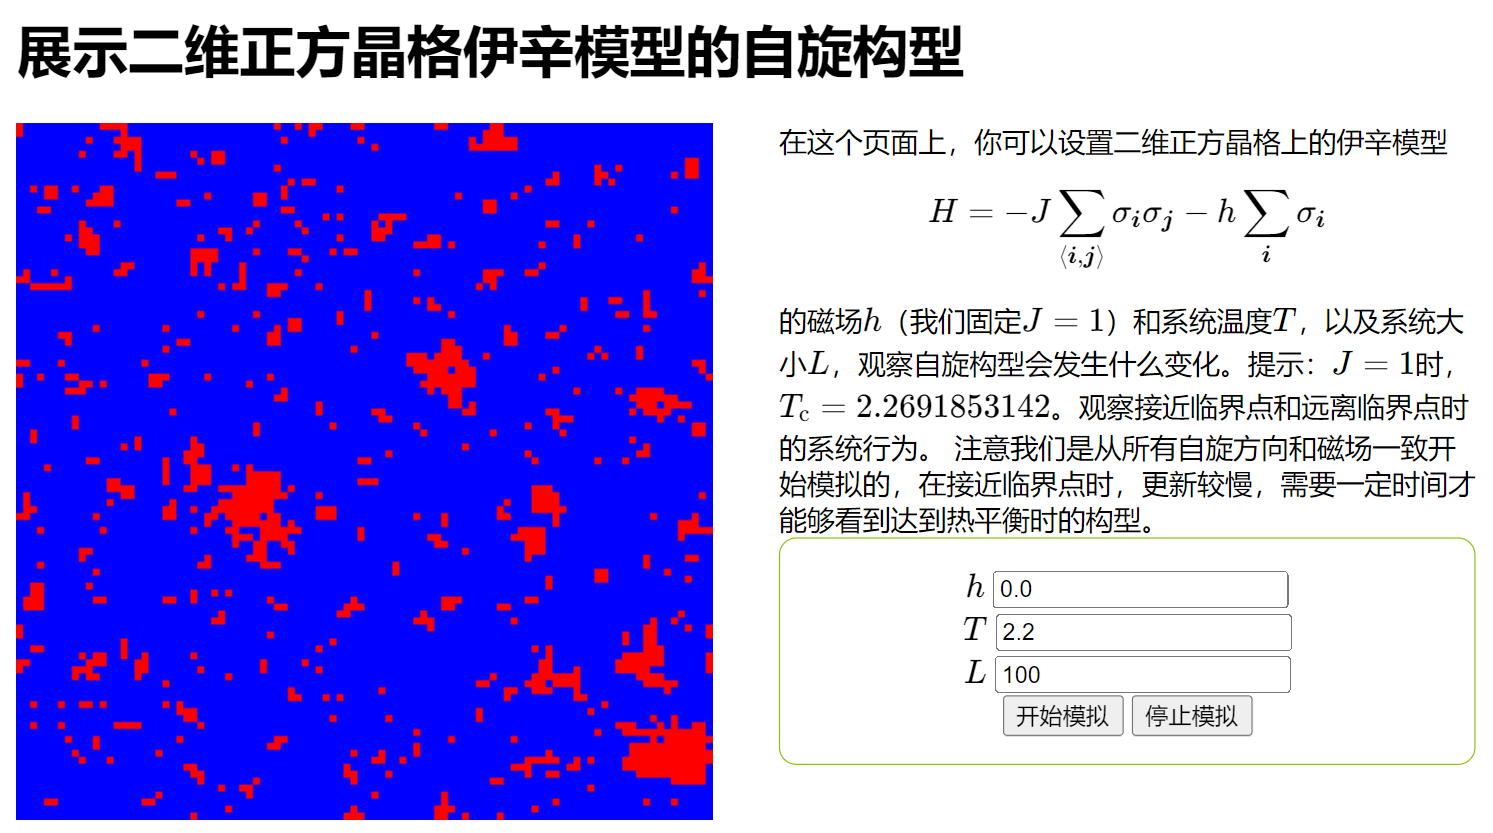
\includegraphics[width=0.6\textwidth]{../ising-report/ising-phase-plot-configuration.PNG}
    \caption{\href{../ising-phase-plot-configuration/index.html}{\texttt{ising-phase-plot-configuration/index.html}}的界面}
    \label{fig:configuration-show}
\end{figure}

运行\href{../ising-phase-plot-configuration/index.html}{\texttt{ising-phase-plot-configuration/index.html}}可以在不同参数下观看二维正方晶格上的伊辛模型的构型的变化情况,其中红色和蓝色分别代表向下和向上的自旋,界面如\prettyref{fig:configuration-show}所示。

\prettyref{fig:examples-ising-configuration}展示了一些不同参数下的自旋构型。可以看到,在$T$明显小于临界温度理论值
\begin{equation}
    T_\text{c} = 2.2691853142
\end{equation}
时(\prettyref{fig:ferro-ising-configuration}),施加一个小的磁场,体系立刻进入同方向的均匀的铁磁态,只有少许热涨落;
在$T$明显大于临界温度时(\prettyref{fig:para-ising-configuration}),体系中向上和向下的自旋出现无规律得到杂乱分布,没有长程序;
$T$接近临节温度时(\prettyref{fig:cluster-ising-configuration}),体系中出现一系列尺度有大有小,各不相同的团簇,大团簇内部有小团簇,将大团簇放大,其内部结构和放大前看起来很相似,说明体系出现了演生的自相似性,这是临界点的典型特征。

\begin{figure}
    \centering
    \begin{subfigure}{0.4\textwidth}
        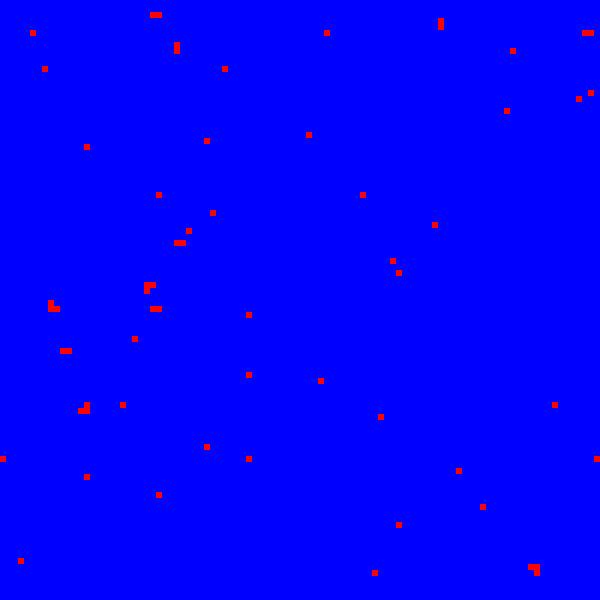
\includegraphics[width=\textwidth]{{../ising-report/T=1.5-L=100-h=0}.png}
        \subcaption{}
        \label{fig:ferro-ising-configuration}
    \end{subfigure}
    \begin{subfigure}{0.4\textwidth}
        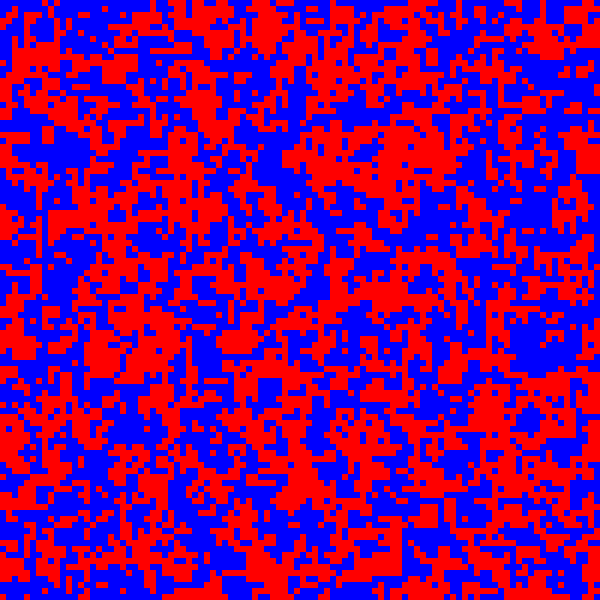
\includegraphics[width=\textwidth]{{../ising-report/T=3.5-L=100-h=0}.png}
        \subcaption{}
        \label{fig:para-ising-configuration}
    \end{subfigure}
    \begin{subfigure}{0.4\textwidth}
        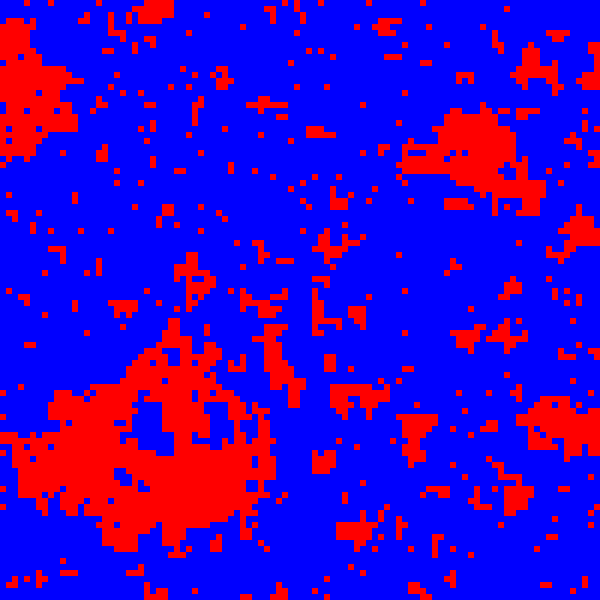
\includegraphics[width=\textwidth]{{../ising-report/T=2.26-L=100-h=0}.png}
        \subcaption{}
        \label{fig:cluster-ising-configuration}
    \end{subfigure}
    \caption{不同参数下的自旋构型,系统边长为$L=100$ (a) $T=1.5, h=-0.1$ (b) $T=3.5, h = 0$ (c) $T = 2.26, h = 0$}
    \label{fig:examples-ising-configuration}
\end{figure}

\subsection{相图扫描演示}

运行\href{../ising-phase-diagram-both-side/index.html}{\texttt{ising-phase-diagram-both-side/index.html}},可以扫描不同边长的体系的相图,界面如\prettyref{fig:phase-diagram-gui}所示。
其中,横轴为$T$,纵轴为$h$,图中每一点都给出了这个参数下的磁化率,青色的点代表自旋全部向下,洋红色的点代表自旋全部向上,两者之间的情况使用蓝色表示。
点击“开始扫描相图”,会看到不同参数处的磁化强度出现在图上。

\begin{figure}
    \centering
    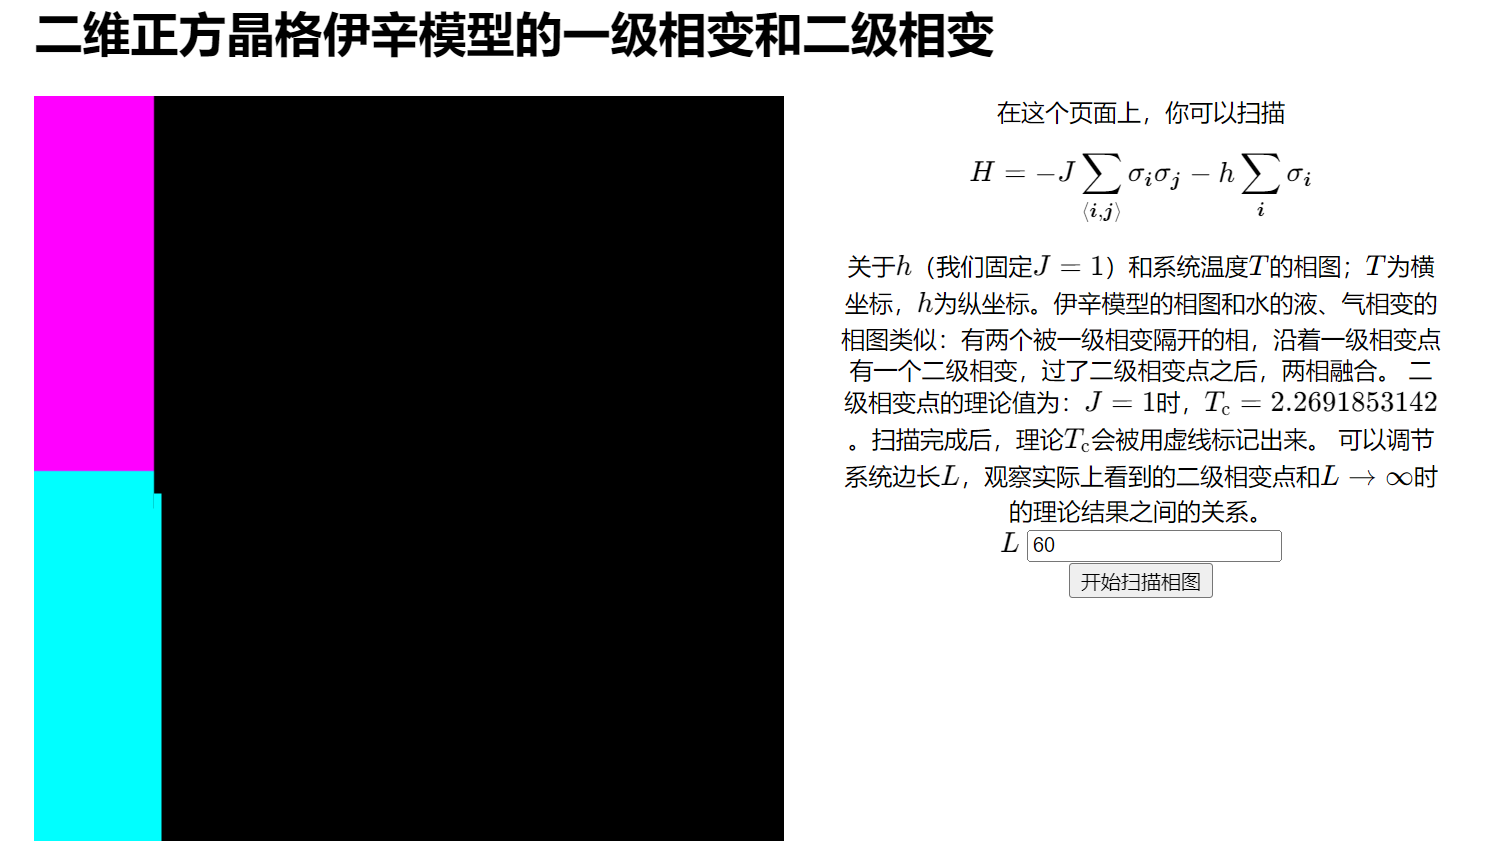
\includegraphics[width=0.6\textwidth]{../ising-report/ising-phase-diagram-both-side.PNG}
    \caption{\href{../ising-phase-diagram-both-side/index.html}{\texttt{ising-phase-diagram-both-side/index.html}}的界面}
    \label{fig:phase-diagram-gui}
\end{figure}

\begin{figure}
    \centering
    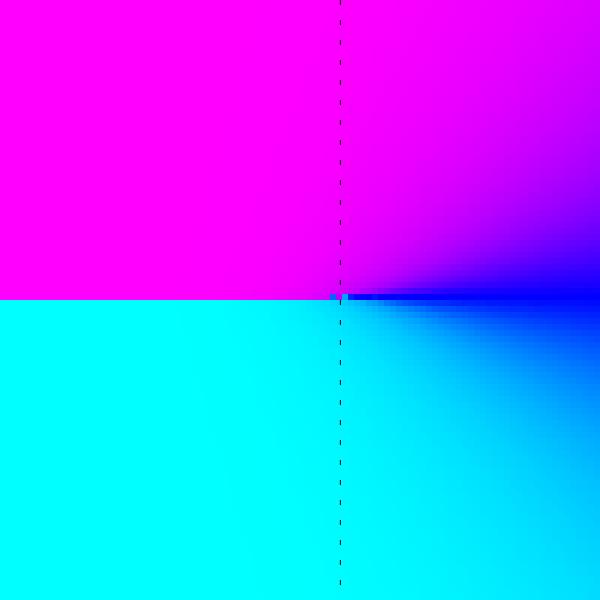
\includegraphics[width=0.4\textwidth]{../ising-report/phase-diagram-L-100.png}
    \caption{$L=100$时数值计算出的相图}
    \label{fig:phase-diagram-example}
\end{figure}

\prettyref{fig:phase-diagram-example}给出了选择$L=100$后计算完成时\href{../ising-phase-diagram-both-side/index.html}{\texttt{ising-phase-diagram-both-side/index.html}}给出的相图,其中的虚线是。可以看到,在$T < T_\text{c}$时,改变$h$会经历从向下的铁磁态到向上的铁磁态的一级相变,但是$T > T_\text{c}$时不存在这个现象。
这暗示我们,沿着$h=0$曲线改动$T$,会经历一个二级相变。
这个相图的结构和水的液相和气相的相图非常类似:两个相被一个一级相变区分,沿着两相交界线经过一个二级相变后,两相融合。%
\footnote{
    固液相变同样有序参量的变化,即晶格结构的出现和不出现,但是这种序参量变化在相变点是不连续的,固液相变因此是一个一级相变,和此处讨论的二级相变不是一回事。
}%

\subsection{相变点处的finite size scaling}

相图上看不清楚二级相变的细节,本节我们根据文献\cite{sandvik2010computational}中提到的方法,对伊辛模型的相变点做所谓的finite size scaling。
一个边长为$L$的系统中的可观测量$Q$可以写成$L$和$T$的函数,或者等价的,$L$和归一化温度
\begin{equation}
    t = \frac{T - T_\text{c}}{T_\text{c}}
\end{equation}
的函数。温度为$T$的无限大系统中的关联长度$\xi$在临界点附近和$t$存在临界指数关系
\begin{equation}
    \xi \sim \abs{t}^{- \nu},
\end{equation}
从而$Q$也可以写成$L$和$\xi$的函数。临界系统通常可以使用较为简单的统计场论描述,其中的场是做过平滑化的序参量$\phi$,而$Q$作为一个意义清晰的物理可观测量,通常形如
\begin{equation}
    Q \sim \int \dd[d]{\vb*{r}} \phi^m (\grad{\phi})^n,
\end{equation}
显然,在临界点上系统具有自相似性,于是$Q$应当具有标度不变性,即如果我们将$L$和$\xi$同时扩大$\lambda$倍,那么$Q$应当是原来的$\lambda^\sigma$倍,其中$\sigma$是某种“反常量纲”,大体上和普通的量纲分析给出的量纲一致但可能因为相互作用修正有一些变动,于是应当能够将$Q$写成以下形式:
\begin{equation}
    Q = L^\sigma f(\xi / L) = L^\sigma f(\abs{t}^{- \nu} / L),
\end{equation}
我们定义一个新函数$g(x) = f(x^{-\nu})$,使得
\begin{equation}
    Q = L^\sigma g(t L^{1 / \nu}).
\end{equation}
$L \to \infty$时$Q$的行为和无穷大系统一致,同样有临界指数关系
\begin{equation}
    Q \sim \abs{t}^{- \kappa},
\end{equation}
于是在$L$较大时只能有
\[
    g(t L^{1 / \nu}) \sim (t L^{1 / \nu})^{- \kappa},
\]
只有这样才能够让$\abs{t}$的指数是正确的。此时
\[
    Q \sim \abs{t}^{- \kappa} L^{\sigma - \kappa / \nu},
\]
由于$Q$不存在$L$依赖了,应有
\[
    \sigma = \frac{\kappa}{\nu}.
\]
于是最后我们得到
\begin{equation}
    Q = L^{\kappa / \nu} g(t L^{1 / \nu}),
\end{equation}
也就是说,将不同的$L$,不同的$T$处的$Q L^{- \kappa / \nu}$和$t L^{1 / \nu}$画在一个坐标系内,我们会发现所有数据点都落在一条曲线上。
这个关系式(以及一系列类似的分析)给出了\emph{有限大小}体系中的标度律,因此称为finite size scaling。

理论上可以证明,二维正方晶格伊辛模型中,磁化率$\chi$和$t$具有如下临界指数关系:
\begin{equation}
    \chi \sim \abs{t}^{- \gamma}, \quad \gamma = 7 /4,
\end{equation}
且二维正方晶格伊辛模型中关联长度的临界指数$\nu$为1,于是取$Q$为$\chi$,$\kappa$为$\gamma$,即可验证磁化率的finite size scaling。
通过简单的统计力学计算可以发现
\begin{equation}
    \chi = \beta L^2 (\expval{m^2} - \expval{m}^2),
\end{equation}
其中$m$为磁化强度,于是可以据此完成$\chi$的“原位”蒙特卡洛测定,而无需真的在不同磁场下做蒙特卡洛计算得到磁化强度再依定义得到磁化率。

由于finite size scaling缺乏物理直观,又需要大量计算,本实验采用Julia编程来实现它。运行
\href{../ising-data-collapsing/ising-data-collapsing/finite-size-scaling-data-generating.jl}{\texttt{ising-data-collapsing/finite-size-scaling-data-generating.jl}},会在程序代码中设定的位置处得到一个包括$L$, $T$, $m$, $\chi$的CSV文件。
据此以及$\nu$,$\gamma$和$T_\text{c}$的理论值绘图,可得到类似\prettyref{fig:finite-size-scaling}的结果。
可以看到,在曲线最大值附近——实际上就是临界点附近,因为$L$固定,变动$T$时,无限大系统中$\chi$会发散,有限大系统中$\chi$会取最大值——数据较为散乱,这是可以理解的,因为Metropolis算法在临界点附近表现不佳。
要获得更好的相变点附近的数据,需要使用集团更新算法。

\begin{figure}
    \centering
    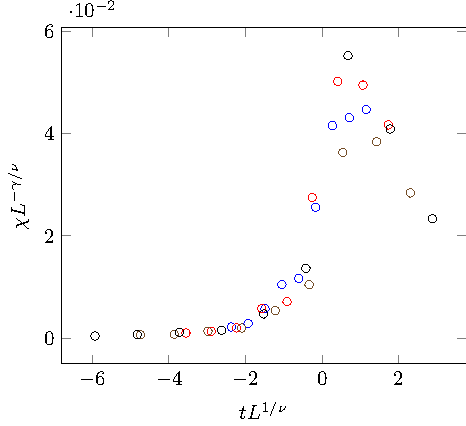
\includegraphics[width=0.5\textwidth]{../ising-report/../ising-data-collapsing/ising-data-collapsing-run-1.pdf}
    \caption{Finite size scaling所得结果示例}
    \label{fig:finite-size-scaling}
\end{figure}

\section{Hubbard模型的行列式蒙特卡洛模拟}

本节讨论Hubbard模型的DQMC模拟。Hubbard模型
\begin{equation}
    H = - t\sum_{\pair{\vb*{i}, \vb*{j}}} c^\dagger_{\vb*{i} \sigma} c_{\vb*{j} \sigma} + U \sum_{\vb*{i}} n_{\vb*{i} \uparrow} n_{\vb*{j} \downarrow} - \mu N
    \label{eq:hubbard}
\end{equation} 
考虑了一个单带、仅有最近邻跃迁的紧束缚模型中的电子的在位(on-site)库伦排斥,是重要的强关联电子模型。
所谓强关联效应是指由于电子间的库伦相互作用,凝聚态系统的行为和基于能带理论的金属/绝缘体行为非常不一致。
就Hubbard模型而言,在$U=0$时,\eqref{eq:hubbard}的能带处于半填充状态,是一个典型的导体。
略微增大$U$会扭曲能带,为了保证电子永远是半填充的,我们在$\mu$和$U$之间施加如下约束
\begin{equation}
    \mu = - \frac{U}{2},
\end{equation}
从而等效的有(忽略一个常数)
\begin{equation}
    H = - t\sum_{\pair{\vb*{i}, \vb*{j}}} c^\dagger_{\vb*{i} \sigma} c_{\vb*{j} \sigma} + U \sum_{\vb*{i}} \left( n_{\vb*{i} \uparrow} - \frac{1}{2} \right) \left( n_{\vb*{i} \downarrow} - \frac{1}{2} \right).
    \label{eq:half-filling-hubbard}
\end{equation}
这个模型具有粒子-空穴对称性,从而其中的电子永远是半填充的。
在这个模型中,如果$U$非常大,由于系统半填充,每个格点平摊到一个电子,如果一个格点上有一上一下两个电子,那么能量就太大了,因此所有电子都被固定在各自的格点上而无法发生跃迁,即不能出现电荷的移动,不过每个格点上的自旋可以翻转。
可以证明,将紧束缚哈密顿量当作微扰后,此时的体系实际上由一个反铁磁海森堡模型描述。
因此,随着$U$的增大,会出现从费米液体到反铁磁绝缘体的转变,这是Mott转变的一个例子,是非常典型的强关联行为\cite{fradkin2013field}。

DQMC是一种常见的处理与Hubbard模型类似的强关联电子模型的蒙特卡洛方法,其基本思想是首先通过离散Hubbard-Stratonovich变换引入一个辅助场,即将有相互作用的费米子理论重写成辅助场背景下的自由费米子理论,然后积掉(integrate out)费米子自由度,得到一个关于辅助场的理论(这个理论中会大量出现行列式,因此这种方法称为“行列式”蒙特卡洛),对这个理论做蒙特卡洛模拟。
由于DQMC涉及大量理论推导,下文中我们将不展示各个公式是如何得到的,而是大致地回顾其思想。有关的细节可见\cite{assaad2008world}等文献。

\subsection{DQMC的基本原理和更新方式}

可以证明对半填充Hubbard模型\eqref{eq:half-filling-hubbard},我们有以下离散Hubbard-Stratonovich变换
\begin{equation}
    \ee^{-\Delta \tau U \sum_{\vb*{i}} (n_{\vb*{i} \uparrow} - 1/2) (n_{\vb*{j} \downarrow} - 1/2)} \simeq \text{const} \times \sum_{s_1, s_2, \ldots, s_n = \pm 1} \ee^{\alpha \sum_{\vb*{i}} s_{\vb*{i}} ({n}_{\vb*{i} \uparrow} - {n}_{\vb*{i} \downarrow})},
    \label{eq:trotter}
\end{equation}
其中
\begin{equation}
    N \Delta \tau = \beta, \quad \cosh(\alpha) = \ee^{\Delta \tau U / 2}.
\end{equation}
依据公式
\begin{equation}
    \trace \ee^{- c^\dagger_i A_{ij} c_j} \ee^{- c^\dagger_i B_{ij} c_j} \cdots = \det(1 + \ee^{- \vb{A}} \ee^{- \vb{B}} \cdots)
\end{equation}
可以积掉费米子自由度,从而配分函数为
\begin{equation}
    Z = \sum_{\vb{s}} Z[\vb{s}], \quad Z[\vb{s}] = \det(1 + \prod_{\sigma=\uparrow, \downarrow} \vb{B}_{\vb{s}}^\sigma(\beta, 0) ),
    \label{eq:dqmc-partition-function}
\end{equation}
其中$\vb{s}$表示将不同$\vb*{i}$和$\tau$点上的$s_{\vb*{i}, \tau}$打包得到的考虑了虚时间维度的辅助场构型,而$\vb{s}_\tau$表示固定虚时间点$\tau$,将不同的$\vb*{i}$处的$s_{\vb*{i}, \tau}$打包起来得到的单个虚时间点的辅助场构型,$\vb{B}$矩阵定义为
\begin{equation}
    \vb{B}^{\sigma}_{\vb{s}}(\tau) = \ee^{\sigma \alpha \diag {\vb{s}_\tau}} \ee^{- \Delta \tau \vb{T}}, \quad \mathbf{B}^\sigma_{\mathbf{s}}\left(\tau_{2}, \tau_{1}\right)=\prod_{n=n_{1}+1}^{n_{2}} \vb{B}^{\sigma}_{\vb{s}}(\tau), 
\end{equation}
其中$\vb{T}$矩阵的两个指标取遍所有格点,$\vb{T}$代表单种自旋的电子的紧束缚模型的一次量子化哈密顿量。
连乘运算$\tau$较大的$\vb{B}$矩阵排在左边。
根据\eqref{eq:trotter},还可以计算出$\vb{s}$给定后的单粒子等时格林函数
\begin{equation}
    \vb{G}^\sigma_{\vb*{i} \vb*{j}}(\tau) = \expval*{c_{\vb*{i} \sigma} c^\dagger_{\vb*{j} \sigma}}_\tau = \left(1+\mathbf{B}^\sigma_{\mathbf{s}}(\tau, 0) \mathbf{B}^\sigma_{\mathbf{s}}(\beta, \tau)\right)^{-1}_{\vb*{i}, \vb*{j}}.
    \label{eq:green-function}
\end{equation}
由于\eqref{eq:trotter}右边的费米子部分是二次型的,在$\vb{s}$给定时,费米子的Wick定理成立,从而,$\vb{s}$给定时,任意复杂的关于电子的可观测量均可通过单粒子格林函数的多项式给出,于是我们对$\vb{s}$做蒙特卡洛采样即可测定任何和电子有关的物理量。

\begin{figure}
    \centering
    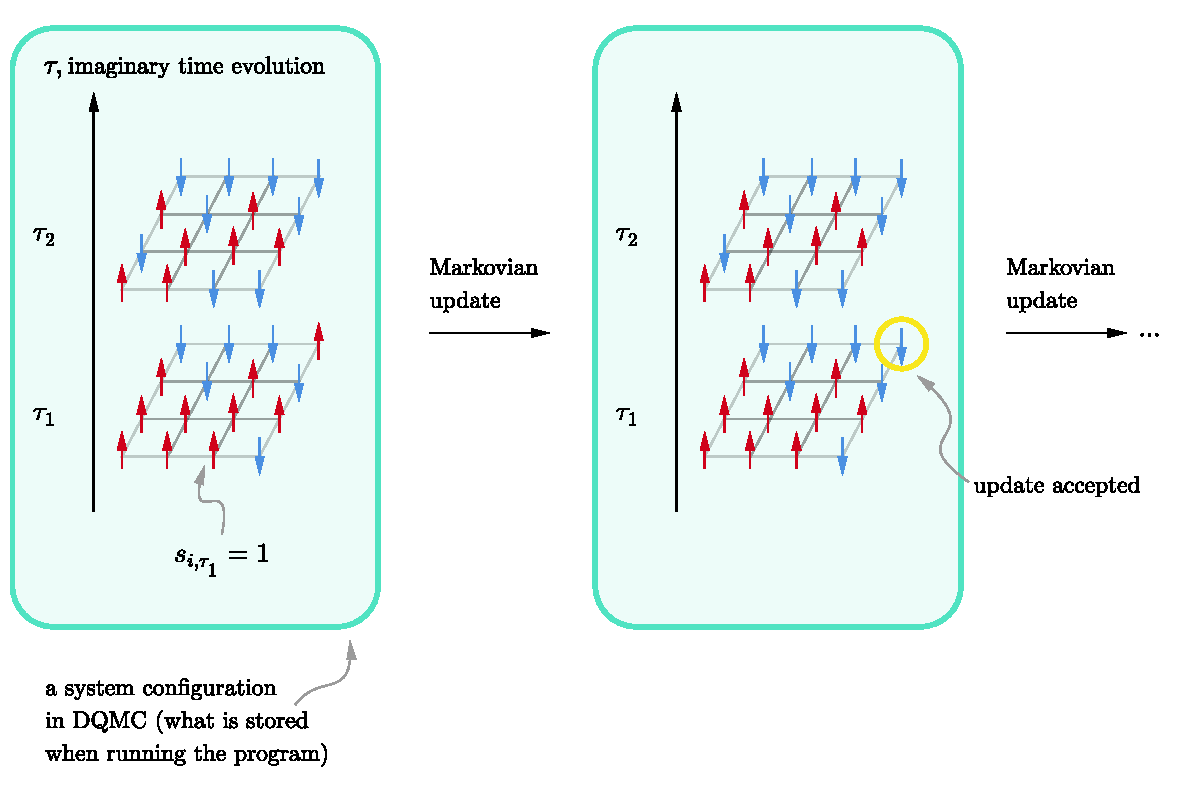
\includegraphics[width = 0.7\textwidth]{../hubbard-report/naive-dqmc.pdf}
    \caption{Hubbard模型的最朴素的DQMC的更新方式}
    \label{fig:naive-dqmc}
\end{figure}

至此我们原则上已经可以做DQMC模拟了:如\prettyref{fig:naive-dqmc}所示,蒙特卡洛程序的内部状态就是$\vb{s}$,更新方式为对$\vb{s}$中的全部自由度——不同$\vb*{i}$,不同$\tau$的$s_{\vb*{i}, \tau}$——做Metropolis翻转,翻转前后的$\vb{s}$的权重由\eqref{eq:dqmc-partition-function}给出,两者的商代入\eqref{eq:metropolis-update}就是接受率。
这样即可正确地对$\vb{s}$的概率分布做采样。要计算电子的物理量的期望值时,使用\eqref{eq:green-function}即可。
例如,双占据的期望值由
\begin{equation}
    \expval*{n_{\vb*{i} \uparrow} n_{\vb*{i} \downarrow}}_{\vb{s}} = (1 - \expval*{c_{\vb*{i} \uparrow} c^\dagger_{\vb*{i} \uparrow}}_{\vb{s}})  (1 - \expval*{c_{\vb*{i} \downarrow} c^\dagger_{\vb*{i} \downarrow}}_{\vb{s}})
\end{equation}
给出。

有若干方法可以优化以上算法的效率。可以证明,翻转$s_{\vb*{i}, \tau}$时的接受率可以用$\tau$时刻单粒子格林函数表示,翻转前后的$\tau$时刻格林函数也有简单的关系,相邻虚时间点的格林函数也可以用$\vb{B}$矩阵联系起来。
因此,费时费力的\eqref{eq:dqmc-partition-function}和\eqref{eq:green-function}可以不必总是进行:\eqref{eq:dqmc-partition-function}实际上从来不需要真的被调用,因为它的作用无非是代入\eqref{eq:metropolis-update}算接受率,而接受率可以用格林函数和不需要求行列式和矩阵连乘的公式得到。
\eqref{eq:green-function}理论上也从来不需要被调用,因为只要在初始化时计算一次格林函数,之后格林函数可以自己更新自己,但为了避免数值误差指数积累,还是需要隔一段时间重新用\eqref{eq:green-function}计算格林函数。
通过解析计算,可以得到和\eqref{eq:green-function}等价但是不需要算矩阵逆的公式,可以大大加快计算。
$\vb{B}$矩阵的构造也有技巧:$\vb{T}$矩阵在计算中从来不改变,从而$\ee^{- \Delta \tau \vb{T}}$可以预先算好;$\diag \vb{s}_\tau$是对角矩阵,计算它的指数是非常简便的。

\subsection{程序结构}

由于DQMC无论如何还是涉及大量线性代数计算,它同样不适宜在HTML5中完成。我们还是使用Julia语言开发Hubbard模型的DQMC程序。%
\href{../hubbard-dqmc/lib.jl}{\texttt{hubbard-dqmc/lib.jl}}包含了做二维正方晶格商的Hubbard模型的DQMC需要的全部程序,将它\texttt{include}到一个Julia环境中即可开始工作。
它能够较为容易地调试和扩展:做DQMC计算时,辅助场构型$\vb{s}$,缓存的$\vb{B}$矩阵等信息被封装在\texttt{HubbardDQMC}结构体中,所有操作——从头开始计算格林函数,计算接受率,做更新等——全部封装在不同的作用在这个结构体上的函数中。
调试时,可以对一个\texttt{HubbardDQMC}结构体做少量操作,观察其变动是否正确。
晶格信息被单独存放在\texttt{HubbardDQMC}的\texttt{lattice}成员中,通过定义每个格点的近邻是哪些格点,即可建立新类型的晶格。
本实验局限于正方晶格,但当然也可以定义三角晶格、六角晶格、Kagome晶格,将它们传入\texttt{HubbardDQMC}结构体中做DQMC模拟。

\href{../hubbard-dqmc/main.jl}{\texttt{hubbard-dqmc/main.jl}}给出了计算不同参数下Hubbard模型的电子动能、双占据和反铁磁序参量的程序。
修改\href{../hubbard-dqmc/config.jl}{\texttt{hubbard-dqmc/config.jl}}可以修改模拟中使用的参数,其中$\texttt{n\_wrap}$指定过多少个虚时间点要按照定义重新计算格林函数。
运行它,控制台输出中将会依次出现模拟使用的参数,各个bin的内部平均值,最后几行输出如\prettyref{fig:main-output}所示,会给出binning结果,即各个物理量在bin间的平均值和标准差。%
\prettyref{fig:hubbard-dqmc-output}给出了\href{../hubbard-dqmc/main.jl}{\texttt{hubbard-dqmc/main.jl}}程序和许霄琰老师的示例程序的比较,表明代码实现无误。
可以看到,随着$U$增大,单电子动能绝对值缩小,由于动能正比于相邻两个格点之间的跃迁的单粒子格林函数,这说明,随着$U$增大,电子越来越难以在格点之间移动了;双占据会减小,即两个电子出现在一个状态上变得越来越不可能了。
这两个结论都和前述Hubbard模型在$U$较大时会出现Mott转变是一致的。

\begin{figure}
    \centering
    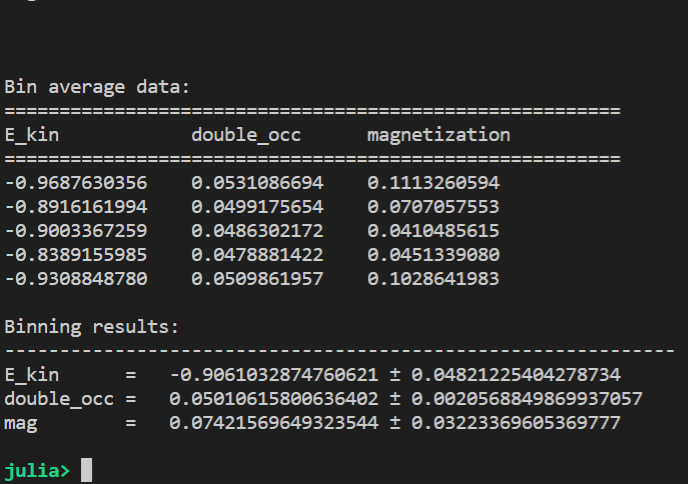
\includegraphics[width=0.6\textwidth]{../hubbard-report/main-result.PNG}
    \caption{\href{../hubbard-dqmc/main.jl}{\texttt{hubbard-dqmc/main.jl}}的控制台输出}
    \label{fig:main-output}
\end{figure}

\begin{figure}
    \centering
    \begin{subfigure}{0.45\textwidth}
        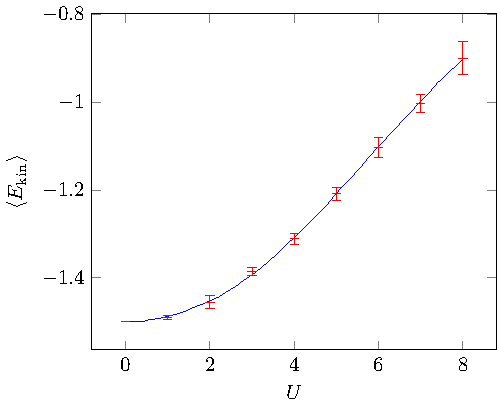
\includegraphics[width=\textwidth]{../hubbard-report/T_compare.pdf}
        \subcaption{}
    \end{subfigure}
    \begin{subfigure}{0.45\textwidth}
        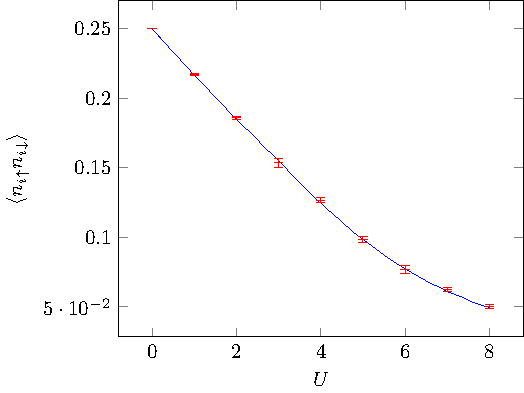
\includegraphics[width=\textwidth]{../hubbard-report/double_occ_compare.pdf}
        \subcaption{}
    \end{subfigure}
    \caption{$L=4$, $\beta = 4$时的物理量计算值(橙色)和许霄琰老师的程序在同样的参数下的输出值(蓝色)的比较 (a) 平摊到每个电子上的动能 (b) 单个格点上的平均双占据}
    \label{fig:hubbard-dqmc-output}
\end{figure}

在晶格做得足够大时,通过格林函数还可以计算不同动量上的电子数分布,从而绘制费米面形状。本实验由于计算资源和时间有限,未能完成此任务。
文献\cite{varney2009quantum}的图2给出了一个示例,其中可以看出$U$增大导致的费米面模糊。

\section{总结与展望}

本实验讨论了伊辛模型和Hubbard模型的蒙特卡洛模拟的原理,使用HTML5和Julia语言,实现了伊辛模型的Metropolis更新,展示了伊辛模型的相图、不同参数下的自旋构型,并讨论了它们的物理意义,绘制了finite size scaling曲线,实现了Hubbard模型的DQMC模拟,绘制了Hubbard模型的电子动能和双占据曲线,并讨论了它们的物理意义。

\bibliographystyle{plain}
\bibliography{monte-carlo}

\end{document}